Before probing for the GC, I first verified that I was able to reproduce the results of Marczak et al.~\cite{Marczak2015} with respect to the GFW.
I then verified that the GFW does not do the same keyword filtering on SSL or TLS traffic.
\subsection{Baseline}\label{gfwbaseline}
This experiment sent the message\\
\texttt{
	\-\ \ \ \ GET /?test HTTP/1.1\textbackslash{}r\textbackslash{}n\\
	\-\ \ \ \ Host: www.google.com\textbackslash{}r\textbackslash{}n\textbackslash{}r\textbackslash{}n\\
}
to IP address \texttt{123.125.65.120:80} via a STREAM socket 24 times, each time with a different TTL value, ranging from 1--24.
This is effectively requesting \texttt{www.google.com/?test} from a server (not Google) in Beijing with connectivity provided by China Unicom (Figure \ref{fig_gfwbaiduip}).
\begin{figure}
	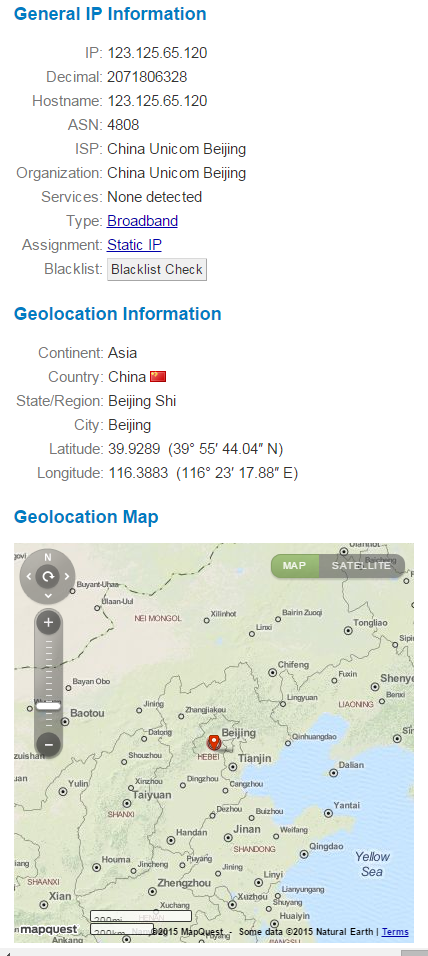
\includegraphics[width=\columnwidth]{figures/gfwbaiduip}
	\caption{
		\cite{IPLookup120} Details on the destination IP address used in the experiments in \autoref{gfwbaseline} and \autoref{gfwlocation}.
		Note the location (Beijing) and the ISP (China Unicom).
	}
	\label{fig_gfwbaiduip}
\end{figure}

All of the requests prompted \texttt{Time-to-live exceeded} messages from intermediary nodes on the way to \texttt{123.125.65.120} until the request sent with TTL=24, which finally gets a \texttt{403} HTTP response (Figure \ref{fig_gfwtest}), as expected when requesting a google.com page from any server other than Google’s.
\begin{figure*}
	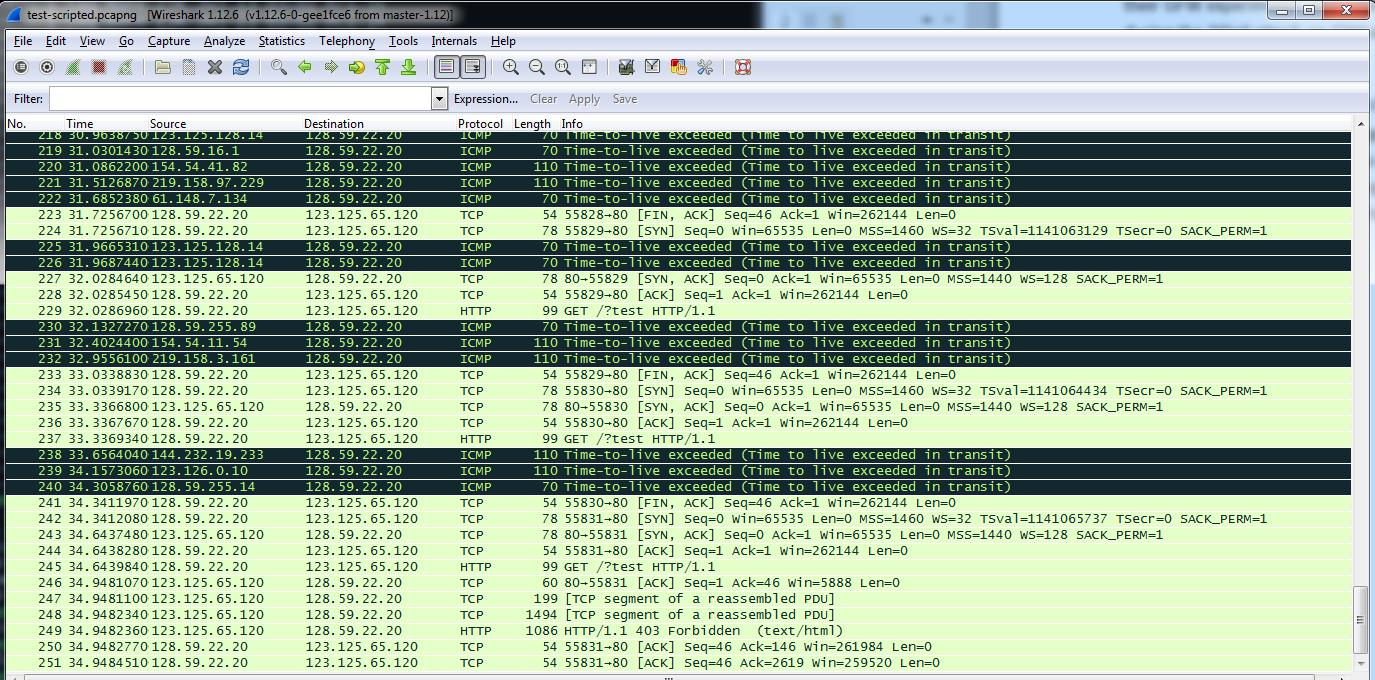
\includegraphics[width=\textwidth]{figures/gfwtest}
	\caption{
		No \texttt{[RST]} packets are sent when \texttt{www.google.com/?test} is requested from a Baidu server in Beijing.
		\texttt{Time-to-live exceeded} messages are received for small TTL values, until an HTTP response is received (packet 249) after sending the request with TTL=24 (packet 245), and the request reaches the Baidu server.
	}
	\label{fig_gfwtest}
\end{figure*}
The full packet capture can be found here: \url{https://github.com/tagatac/ttlprobe/blob/prelim/test-scripted.pcapng}.
The one spurious \texttt{[RST]} packet (packet 87) sent from my computer to \texttt{123.125.65.120} is a closing connection from a previous run of the same experiment.
You can see this from the port number used (55785), which is out of sequence with those from this experiment (55805--55831).
\subsection{GFW Location}\label{gfwlocation}
This experiment shows that the GFW is between 17 and 18 hops from my desktop along the path to \texttt{123.125.65.120}.
An identical experiment to Experiment 1 was performed, only substituting \texttt{falun} for \texttt{test} in the HTTP \texttt{GET} requests.
The results are the same as in \autoref{gfwbaseline} for TTL values 1--17.
For each TTL$\geq$18, I received an \texttt{[RST]} packet and three \texttt{[RST, ACK]} packets apparently from \texttt{123.125.65.120} (but actually from GFW).
\texttt{[RST]} packets sent by the GFW to both endpoints (my desktop and the server and \texttt{123.125.65.120}) cause both to close the TCP connection.
The packet capture can be found here: \url{https://github.com/tagatac/ttlprobe/blob/prelim/falun-scripted.pcapng}.
The script used for both the experiments in \autoref{gfwbaseline} and \autoref{gfwlocation} can be found here: \url{https://github.com/tagatac/ttlprobe/blob/prelim/test.py}.
Figure \ref{fig_gfwfalun} shows the request with TTL=18 prompting the first \texttt{[RST]} packet from the GFW.
\begin{figure*}
	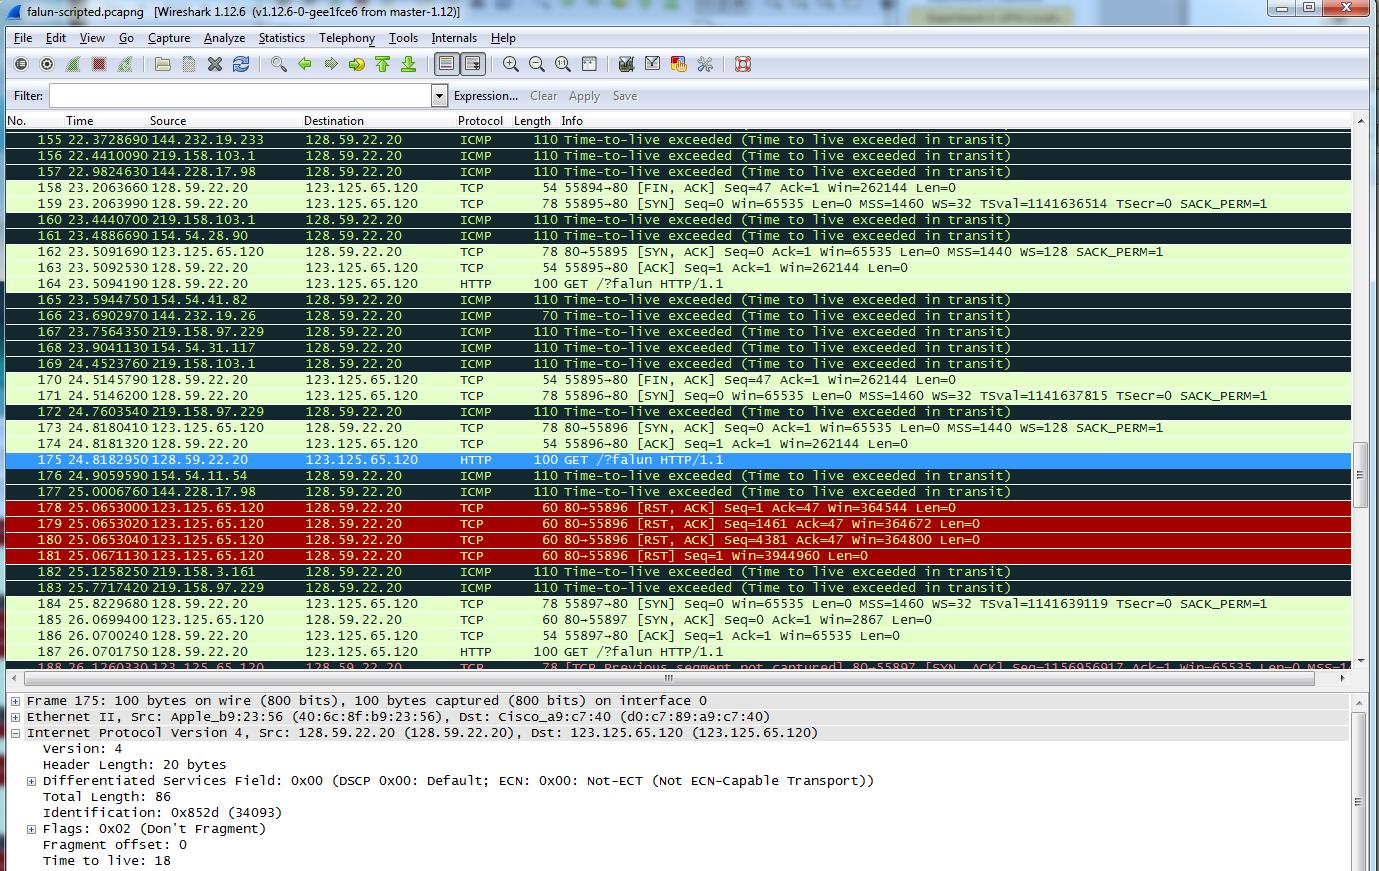
\includegraphics[width=\textwidth]{figures/gfwfalun}
	\caption{The GFW responds to the keywords \texttt{www.google.com/?falun} with several \texttt{[RST]} packets as soon as the request is sent 18 hops along the path to a Baidu server in Beijing.}
	\label{fig_gfwfalun}
\end{figure*}
\subsection{Probing for Keyword Filtering On \allowbreak{}Encrypted Traffic}\label{gfwtls}
In a similar way to \autoref{gfwlocation}, I probed for keyword filtering on HTTP requests sent to servers in China, but this time with encrypted TCP packets.
Note that many Chinese websites maintain servers in Hong Kong, or elsewhere outside of mainland China, so that DNS servers in the U.S. resolve those domains to servers that are not behind the GFW.
In order to identify a Baidu server in China, I instead used a Chinese DNS server \texttt{115.28.245.152} located in Hangzhou, which I obtained from a site which lists public DNS servers~\cite{PublicDNS}.
Using this server resolves \texttt{www.baidu.com} to \texttt{CNAME www.a.shifen.com} and IPv4 addresses \texttt{220.181.112.244} and \texttt{220.181.111.188}, both of which are located in Beijing according to geolocation databases~\cite{IPLookup244,IPLookup188}.

A \texttt{tcptraceroute}~\cite{Toren2006} identifies the first IP address \texttt{220.181.112.244} as being 22 hops away from my desktop.
A repeat of the experiment in \autoref{gfwlocation} (with unencrypted TCP packets) to this IP address shows that, as expected, requests for \texttt{www.google.com/?falun} sent with TTL values of at least 16 are detected by the GFW, and \texttt{[RST]} packets are received.
The packet capture can be found here: \url{https://github.com/tagatac/ttlprobe/blob/tlsprobe/pcaps/falun-220.pcapng}.

Then three more probes were performed.
These probes sent the following requests with the specified encryption, and TTL values ranging from 0--24:
\begin{enumerate}\addtolength{\itemsep}{-.35\baselineskip}
	\item \texttt{www.google.com/?test} sent over TLS1.2
	\item \texttt{www.google.com/?falun} sent over TLS1.2
	\item \texttt{www.google.com/?falun} sent over SSL3
\end{enumerate}
Not one of these requests generated an \texttt{[RST]} packet from the GFW.
The script used to these probes can be found here: \url{https://github.com/tagatac/ttlprobe/blob/tlsprobe/probe.py}.
It uses the standard Python libraries \texttt{socket} and \texttt{ssl}, wrapping a socket connection with the appropriate (TLS1.2 or SSL3) \texttt{ssl.Context}.
The packet captures for these probes can be found at the following respective URLs:
\begin{enumerate}\addtolength{\itemsep}{-.35\baselineskip}
	\item \url{https://github.com/tagatac/ttlprobe/blob/tlsprobe/pcaps/test-220-tls.pcapng}
	\item \url{https://github.com/tagatac/ttlprobe/blob/tlsprobe/pcaps/falun-220-tls.pcapng}
	\item \url{https://github.com/tagatac/ttlprobe/blob/tlsprobe/pcaps/falun-220-ssl.pcapng}
\end{enumerate}
The certificate offered by the server at texttt{220.181.112.244} can be found here: \url{https://github.com/tagatac/ttlprobe/blob/tlsprobe/baiducert.pem}.

These results support the hypothesis that the GFW does \textit{not} perform keyword filtering on encrypted traffic.